\section{Experimental evaluation}
% 1. Compare performance
%   - Finetune 2M steps and observe the curves of default/learnable_skill_weight/fair_weight/fixed_one_weight
% 2. Compare sample efficiency
%   - Finetune 100k steps and observe the final performances of default/fair_weight

% Introduce an environment
% 환경에 대한 전반적인 소개
We experimented proposed methods on URLB \cite{laskin2021urlb}, which contains three continuous control environments and twelve downstream tasks.
The environments include 6-DOF \emph{Walker}, 12-DOF \emph{Quadruped}, and 9-DOF \emph{Jaco arm}. 

\begin{figure}[ht]
    \vskip 0.2in
    \begin{center}
    \centerline{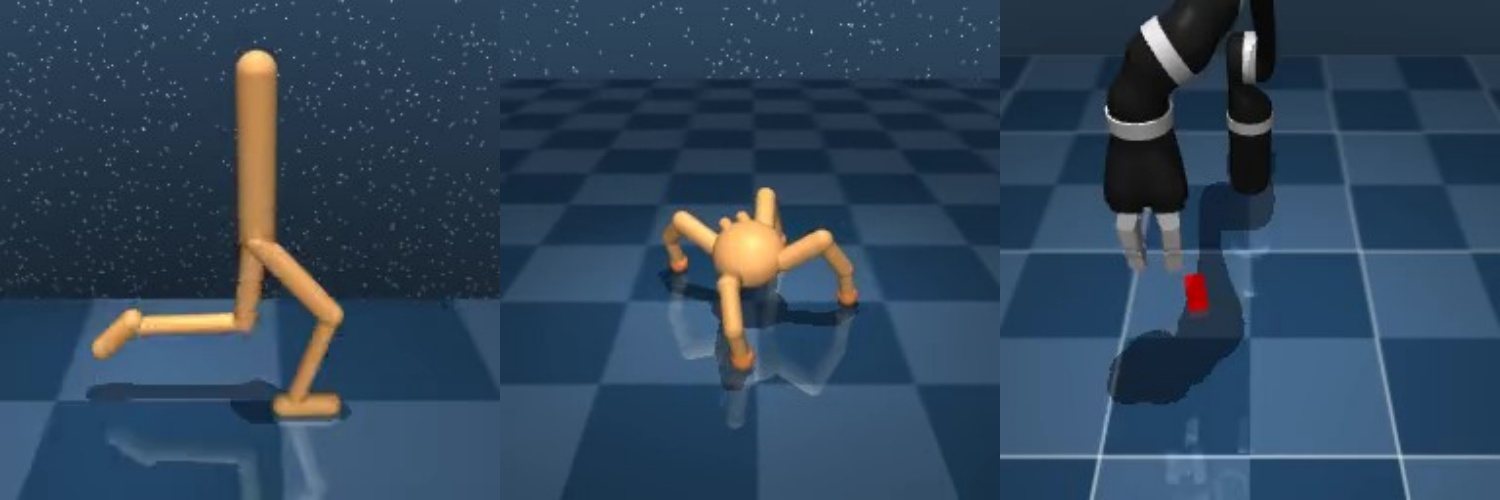
\includegraphics[width=\columnwidth]{Figures/figure_env.jpg}}
    \caption{Continuous control environments from DeepMind Control Suite. Left: Walker, center: Quadruped, right: Jaco arm.}
    \label{fig:environments}
    \end{center}
    \vskip -0.2in
\end{figure}


There are two phases in URLB.
The first phase is a reward-free pre-training phase and the other is fine-tuning phase with explicit rewards.
In a reward-free environment, methods such as DIAYN train the agent to understand the environment with intrinsic rewards.
In case of skill discovery method, the agent learns a set of useful behaviors which we call skill.
Then we use these skills to get higher return (cumulative rewards) quickly in fine-tuning.
% Our method suggests several methods to combines these skills together and shows great performance.
When we evaluate our methods, we fix the pre-trained agent as DIAYN and fine-tuned in various ways.


\begin{figure}[ht]
    \vskip 0.2in
    \begin{center}
    \centerline{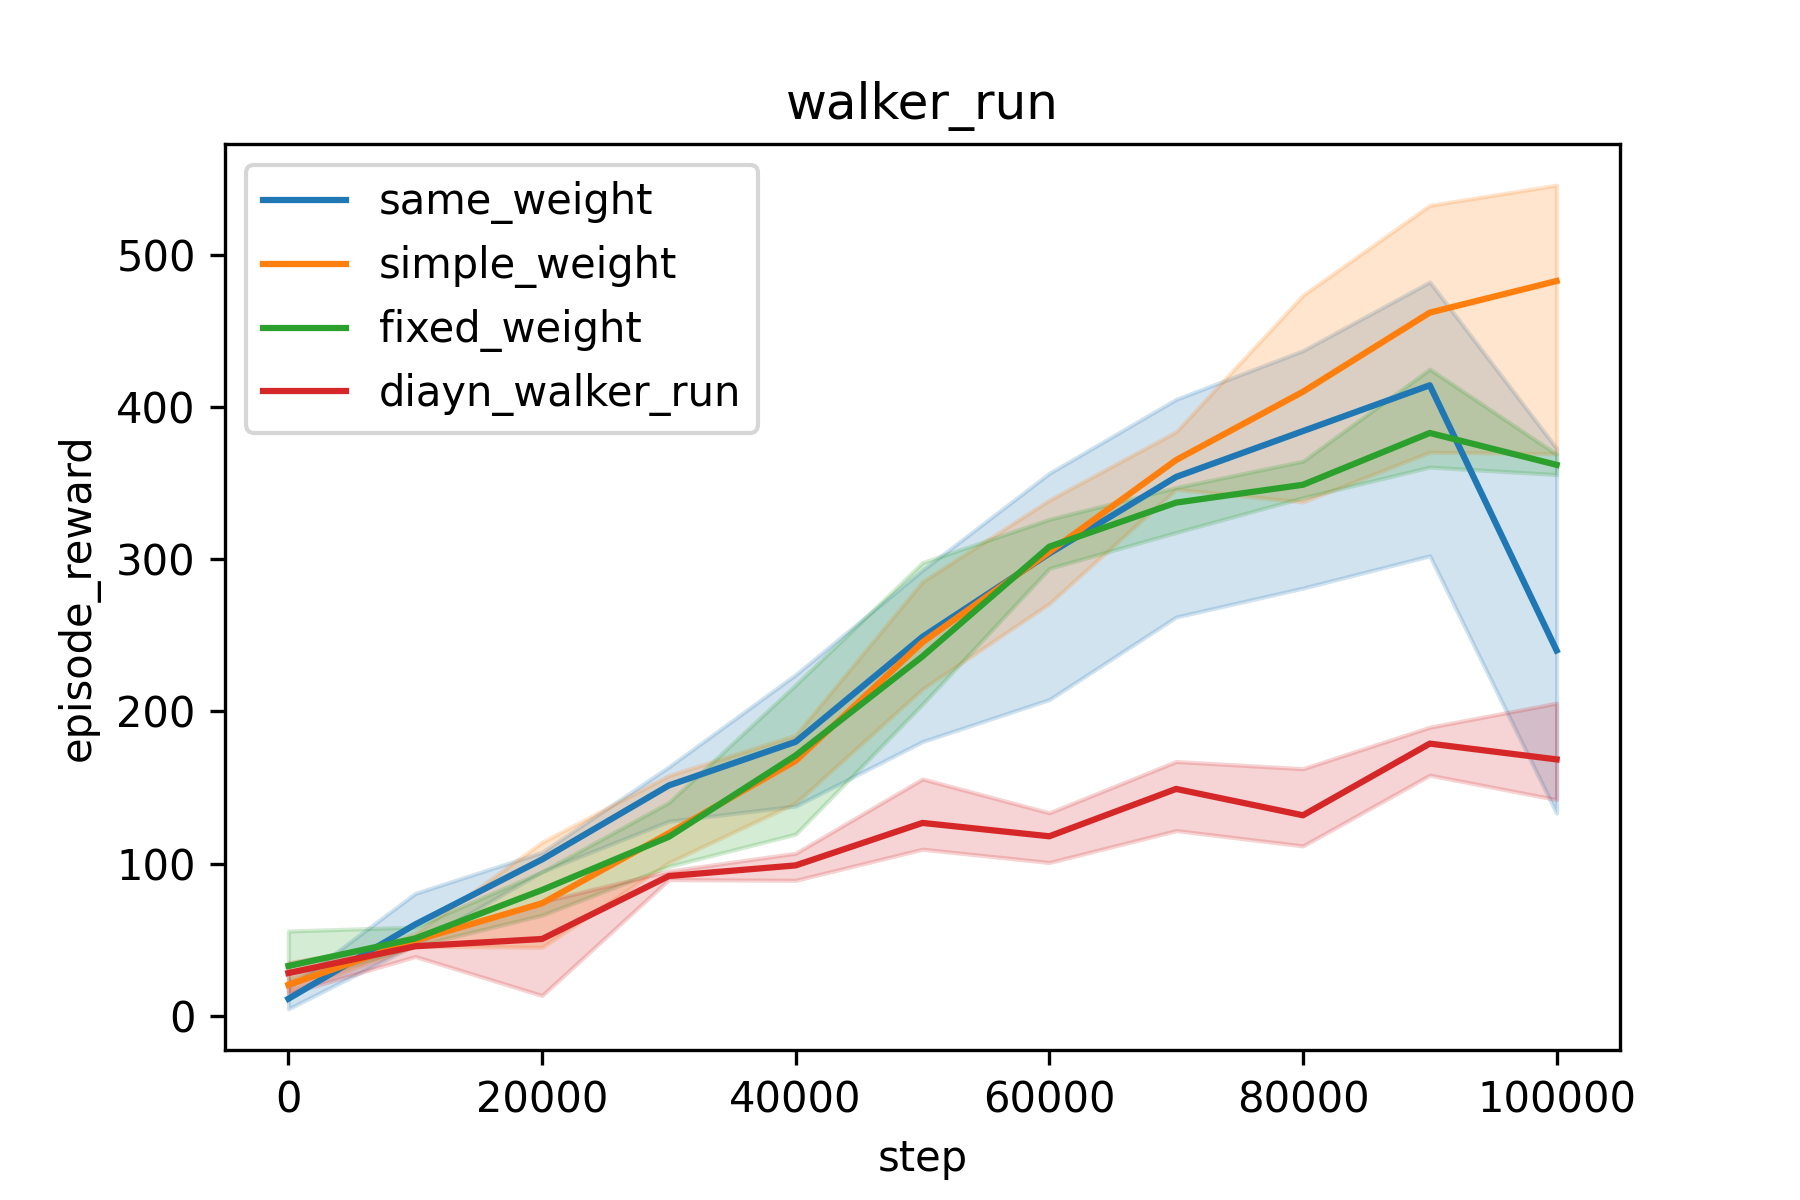
\includegraphics[width=\columnwidth]{Figures/multiple_seed_state_agnostic_methods.png}}
    \caption{Finetuning results of state agnostic skill weight methods. Same skill importance method achived the best result.}
    \label{state agnostic results}
    \end{center}
    \vskip -0.2in
\end{figure}

% Looking at the final learned ${w_i}$, it can be seen that all perspectives are used near evenly.


\subsection{Evaluation for Performance}
% walker-run에서 결과 비교 (100k steps or 2M steps?)
% 분량 제한때문에 state-agnostic과 skill-dependent skill 실험을 하나로
% 2M step, 3 seeds로 default diayn, learnable, same weight, fixed one weight,
% skill-dependent skill까지 하나의 plot으로 만드는게 나을듯

% 실험 세팅 설명
\subsubsection{State agnostic method}
We compare our methods to default DIAYN fine-tune method implemented in URLB.
We choose the task Walker-run for the comparison because it is the most challenging task among the twelve downstream tasks in URLB.
We use a same pre-trained DIAYN policy for a fair comparison, and fine-tune each method for 100k steps.
All the methods are trained in end-to-end manner using DDPG which is a default fine-tuning method in URLB.
\emph{Default DIAYN} is a default fine-tuning method which is implemented in URLB that fixes $p(z)$ as uniform distribution in equation \ref{action-fuse-eq} and only fine-tune a skill-based policy $\pi(a|s,z)$.
\emph{Learnable weight} and \emph{Fair weight} are both state-agnostic fusion methods, but the former fine-tunes $p(z)$ and latter fixes.

The parameters for these method serve to fuse the state viewed from various perspectives to help the agent obtain the optimal reward in a faster way.
\emph{Fixed one weight} fine-tunes only for one best skill. As mentioned in Section \ref{section:method}, it costs for selecting the best skill,
but we did not count the process in as a step to make a baseline more challenging. The default DIAYN method is blue line on \cref*{state agnostic results}, and all other methods exceed this baseline.

% 결과 해석
% 사실 우리가 원하는 바는 fixed_one_weight의 성능이 나쁜 것인데...
% 결과가 나온 후에 해석을 잘 붙여보자
We believe this result came about for two reasons.
First, because the default DIAYN finetunes uses only one skill per episode.
This has disadvantage of not being able to utilize other skills learned during pretraining.
Secondly, the sampled skill is not optimal with high probability.
Since there's no way default DIAYN finetuning know which skill is good for the downstream task,it samples the skill uniformly.
And this uniform sampling of course highly not optimal.
This may be useful if interpreted as a method of obtaining a general agent in multi-task learning,
but it is inappropriate as an approach that aim to achieve maximum performance in a specific goal-oriented downstream task.
In fact, using only one fixed skill which is chosen at random far exceeds default DIAYN implemented in URLB.(Red line)
This reveals that randomly changing skill at finetuning phase harms a performance a lot.

% In \cref*{final_skill_weight}, we can check the agent use skills near evenly.
% This allows for faster and better performance, as shown in the \cref{finetuning result}.
\begin{figure}[ht]
  \vskip 0.2in
  \begin{center}
  \centerline{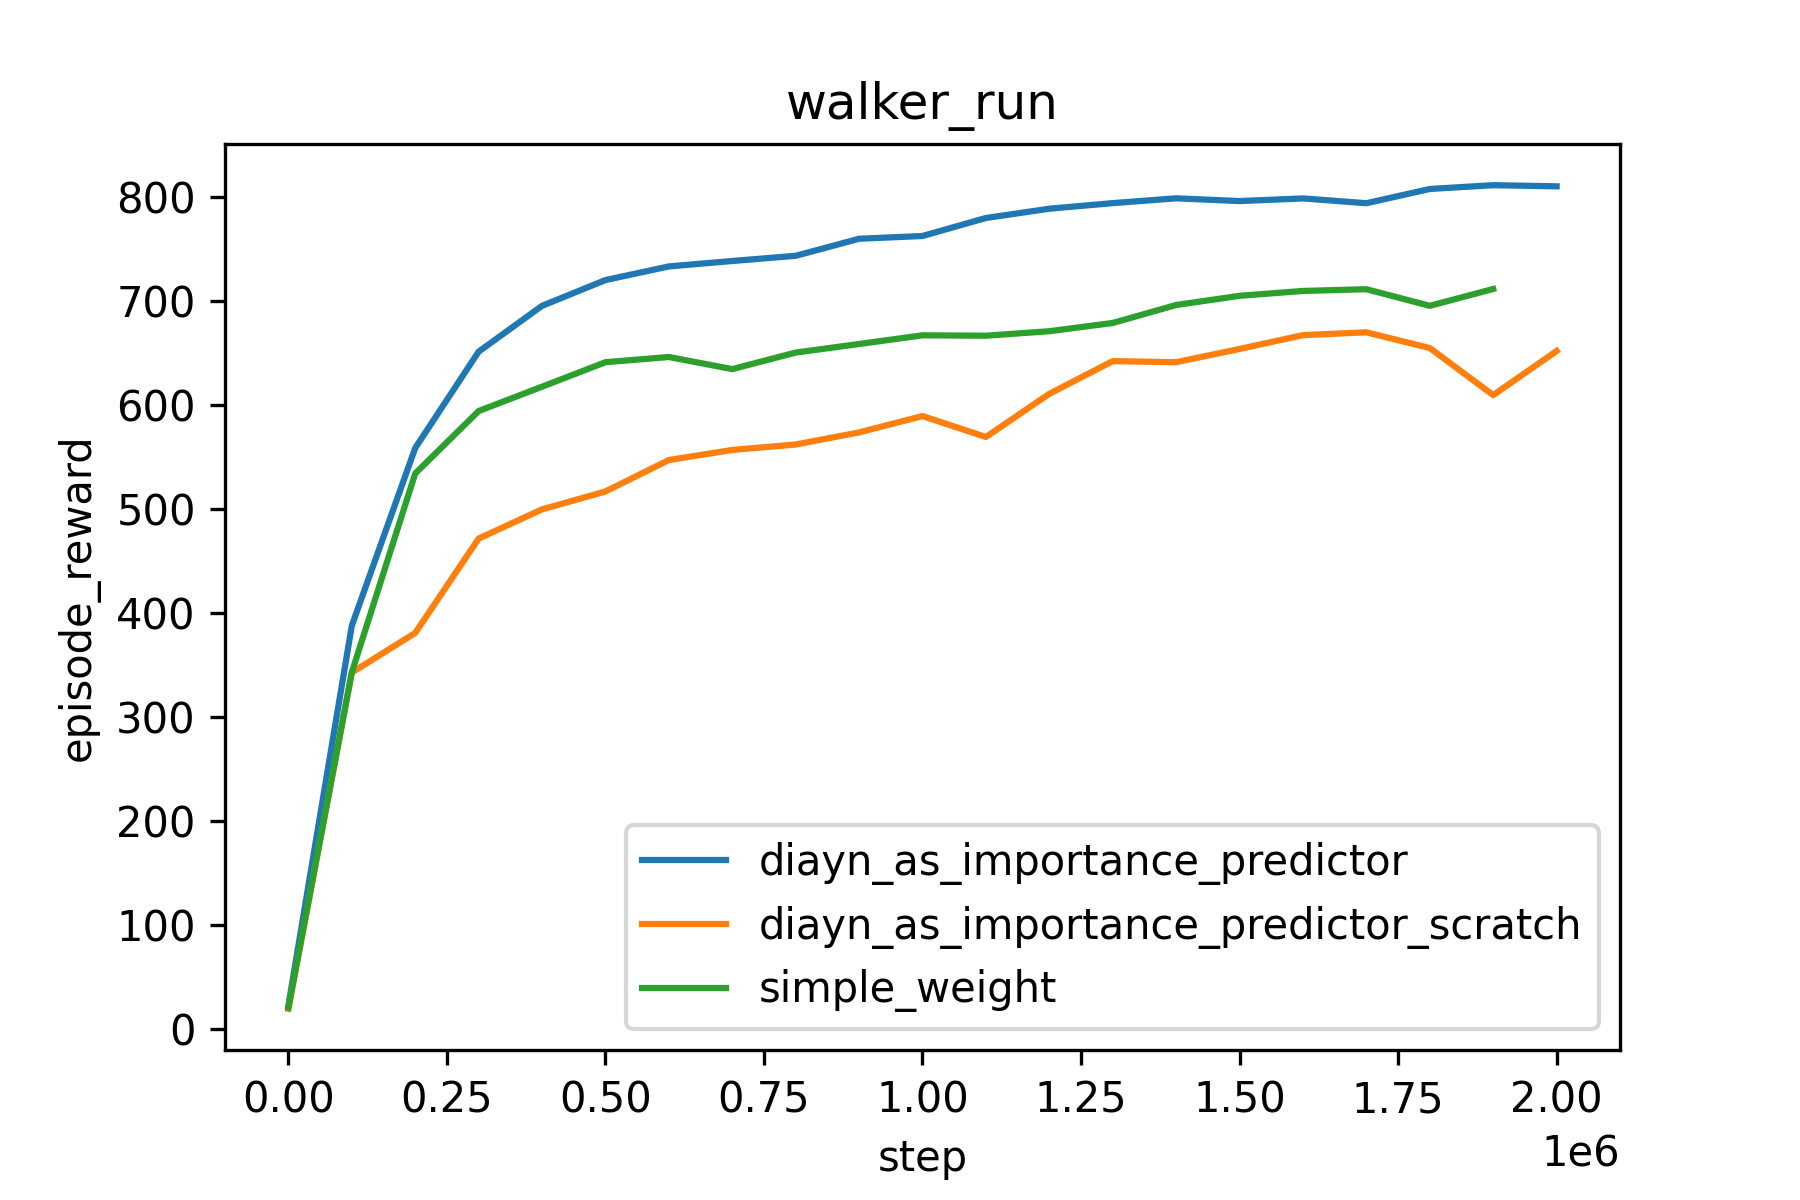
\includegraphics[width=\columnwidth]{Figures/diayn_as_importance_predictor.png}}
  \caption{State agnostic methods showed faster learning, but state aware method achieved better result at the end.}
  \label{diayn-as-skill-weight}
  \end{center}
  \vskip -0.2in
  \end{figure}


%%% 여기서부터는 원래 다른 실험 (2M finetune)
% \subsection{DIAYN as skill weight predictor}
\subsubsection{State agnostic method}
The second is to use the DIAYN module used in the pretrain phase as a skill weight predictor.

% \subsubsection{Weight transfer from pretrained DIAYN}
With the transfered weight from pretrained phase, DIAYN module learns to output the skill weight in end to end manner.
However, the learning results were not good.
There was a part where the performance deteriorated significantly for a certain period..
% \subsubsection{Train from scratch}


%%% URLB와 same weight 비교하는 실험
% 100k fine-tuning
\subsection{Evaluation for Sample Efficiency}
We evaluate how quickly the agent adapt to the downstream task in the same setting to URLB \cite{laskin2021urlb}, 2M pre-train steps and 100k fine-tune steps.
Among our proposed methods, as we have seen on the experiment above, \emph{same weight} method is the most sample efficient.
Therefore, we fine-tune pre-trained DIAYN with \emph{same weight}  for 3 seeds per task.
We compared our method with 9 unsupervised RL algorithms including DIAYN with a vanilla fine-tuning.
Expert performance is a DDPG result after 2M steps of fine-tuning \cite{laskin2022cic}.
Other best is a state-of-the-art among twelve unsupervised RL reported in URLB.

As shown in Table \ref{table:result_urlb}, although the simple fine-tune method without any additional weight is applied,
it outperforms every other methods in 9 out of 12 tasks.
Even for the tasks that other methods work better(Quadruped-stand, Jaco-reach-bottom-right, Jaco-reach-top-right),
out method just slightly underperforms.
Especially, it achieves an enormous improvement compared to the reported original DIAYN.
From this experiment, we can recognize how important the fine-tuning method is for
evaluating a skill discovery methods.

% To follow the comparison introduced in URLB \cite{laskin2021urlb}, 2M steps are pretrained and then 100k steps finetuning is performed.
% Our method outperformed the other unsupervised RL methods in 12 environments and the result is summarized on table \ref{table:result_urlb}.
% It is noteworthy that the simplest state agnostic skill weight method among our proposed methods obtained the best performance. 




% \subsection{MultiHeadAttention to attain several skill weight}
% Third, we use MultiHeadAttention to have multiple the skill weights.
% The result was fine.
% However, there is not much gain compared to Simple Weight.
% In this case, using simple weights is parameter efficient.

% \subsubsection{self attention}
% \subsubsection{use state as query attention}

% \subsubsection{Fixed one skill}
% \subsubsection{Sampling skill(DIAYN)}

% \subsubsection{Zero skill weight}
% We came to a question when we saw that skill weight was evenly distributed.
% If we take average of ${[s,z]}$ vectors, isn't it the same as just having state without skill?
% This is because the more evenly the importance is distributed, the closer the skill vector is to 0 vector in one-hot vector. Figure needed?
% This is because, when concating, the mean of state vector part will be same as the original value,
% but the skill vector part will be a near-uniform distributed vector of about $\frac{1}{skilldim}$.
% This makes it doubtful whether the skill vector part has any meaning.

% If weighted skill vector has really no meaning, then the agent without skill should outperform our method.
% Therefore, we compare our method with DDPG + DDPG agent. The result is that our method is better.

% This reveals that the skill allows it to learn some meaningful behavior.
% Maybe the skill distribution looks like a flat, meaningless vector to our eyes, but the slight difference is meaningful.
% If weighted skill vector has really no meaning, then the agent without skill should outperform our method.
% Therefore, we compare our method with DDPG + DDPG agent. The result is that our method is better.

% This reveals that the skill allows it to learn some meaningful behavior.
% Maybe the skill distribution looks like a flat, meaningless vector to our eyes, but the slight difference is meaningful.